\documentclass[]{IEEEtran}
\usepackage[utf8]{inputenc}		%UTF8 input file
\usepackage[T1]{fontenc}		
\usepackage[ngerman]{babel}
\usepackage{amsmath, amssymb}
\usepackage{eurosym}
\usepackage{hyperref}
%Für Fußzeilten
%\usepackage{stfloats}
%Bilder
\usepackage{graphicx}

%Zeilenabstände
\usepackage{setspace}


\title{Pflanzengießanlage}
%\subtitle{DIY14Pflanze}
\date{\today}
\author{ Stefan Schubäck, \and Matthias Nagl,\and Christoph Hofbauer, \and Dmitrii Cetvericov, \and Markus Fischer-Has,}

%\renewcommand{\iedlistdecl}{\settowidth{\labelwidth}{Hello}}

\begin{document}


	\maketitle
%	\tableofcontents

\begin{abstract}
Auch unter den Studenten gibt es den einen oder anderen mit einem grünen Daumen, der seine Wohnung durch ein paar Pflanzen aufgewertet hat. 
Wenn nicht das ständige Gießen wäre. 
Vor jedem längeren Urlaub stellt sich die Frage, was machen mit den Pflanzen? 
Den Nachbarn fragen und hoffen er ist da und verlässlich? 
Die Pflanzen \glqq Absaufen\grqq \ lassen und hoffen, dass die sich das Wasser einteilen? 
Beides keine zufriedenstellende Lösung. Wieso lässt man sich die Pflanze nicht selber gießen?
Aus diesen Überlegungen ist die Idee entstanden, eine Pflanze mit Sensoren auszustatten, die uns über den aktuellen Zustand informieren. 
Im Folgenden wird der Aufbau zweier Lösungen vorgestellt. 
Der erste Ansatz basiert auf dem Arduino-System, dass einen einfachen Einstieg in Umgang mit Mikrocontroller ermöglicht. 
Der zweite Ansatz baut auf ähnliche Hardware ohne die Verwendung der Arduino Software Programmierumgebung. 
Dadurch wird die Verwendung von Sleep"~Modi und Interrupts möglich was somit zu einer Low"~Energy Variante des Gießsystems führt.  

\end{abstract}

\section{Eingrenzung}
Es lassen sich viele Faktoren finden, die einen Einfluss auf das Wohlbefinden eine Pflanze haben. 
Hierunter fallen die Bodenfeuchtigkeit im Topf der Pflanze, die durchschnittliche Sonneneinstrahlung, der Luftqualität, der Nährstoffgehalt des Bodens sowie die Temperatur an der Wurzel der Pflanze. 
Diese nicht abschließende Aufzählung zeigt, dass eine Eingrenzung der zu untersuchenden Faktoren notwendig ist um das Projekt in der gegeben Zeit fertigzustellen.
Auch in Hinblick des Einsatzgebietes gibt eine Vielfalt von unterschiedlichen Möglichkeiten wie z.B. Einpflanzenbetrieb oder Mehrpflanzenbetrieb sowie Indoor oder Outdoor. 
Im Rahmen des Projekts werden demnach folgende Eingrenzung vorgenommen:

\begin{itemize}
	\item Die Bodenfeuchtigkeit wird abgeleitet aus der Widerstandsänderung einer Messgabel die sich im Erdreich der Pflanze befindet. Die Widerstandsänderung ergibt sich aus der Änderung des Wassergehalts der Erde.
	\item Das System soll für eine alleinstehende Pflanze aufgebaut werden. 
	\item Das Einsatzgebiet wird im Innenbereich sein. Dadurch fallen Einschränkungen bzgl. Witterungs"-beständigkeit weg.
	\item Die Stromversorgung wird über ein Netzteil bewerkstelligt. 
	\item Das System soll über eine Drahtlose Verbindung einstellbar sein. Diese Einschränkung gilt nur für die Arduino Variante, da in der Sparversion auf die Kommunikation verzichtet wird. Hier wird die Einstellung direkt im Code vorgenommen.

\end{itemize}

Weitere Ideen wie z.B. eine Autarke Lösung mit Batteriebetrieb, ein Mehr"~Pflanzenbetrieb oder ein System für den Garten wurden zwar diskutiert, aber wegen dem erhörten Zeitaufwand und begrenzten Budgets nicht weiter verfolgt. 
Im folgenden wird die \emph{Arduino Version} ausführlich vorgestellt. 
Die \emph{Sparversion} wird im Anschluss erläutert, da viele der Funktionen grundsätzlich identisch sind wird darauf verzichtet diese erneut auszuformulieren. 

%section
\section{Arduino"~Variante}

In Abbildung \ref{fig-SchemaAufbau} ist der schematische Aufbau des Projektes zu sehen. Das Gießsystem besteht aus der Steuereinheit, dem Wasserbehälter sowie der Pumpe mit dem Schlauchsystem. Aus dem Steuergerät wird der Sensor über einen Cinch"~Anschluss herausgeführt. Auf der linken Seite wird das Netzteil mit einem Hohlstecker verbunden. 
Im Folgenden beschreiben wir das Vorgehen für das Gießsystem basierend auf der \emph{Arduino"~Variante}. 
Es wird hierzu auf folgende Bereiche eingegangen:

\begin{itemize}
	\item Zu Beginn beschreiben wir verschiedenen Möglichkeiten des Wassertransports zur Pflanze.
	\item Im weiteren stellen wir das Vorgehen zur Erstellung des Gehäuses für die Elektronik dar.
	\item In Abschnitt Elektronik werden wir auf den Aufbau der Platine und die hiermit verbunden Bereiche \emph{Sensorik}, \emph{Kommunikation} und \emph{Stromversorgung} eingehen.
	\item Anschließend wird das Programm für den Mikrocontroller beschrieben.
	\item Abschließend wir ein Kostenplan vorgestellt. 
	
\end{itemize}

	\begin{figure}[ht]
	\centering
	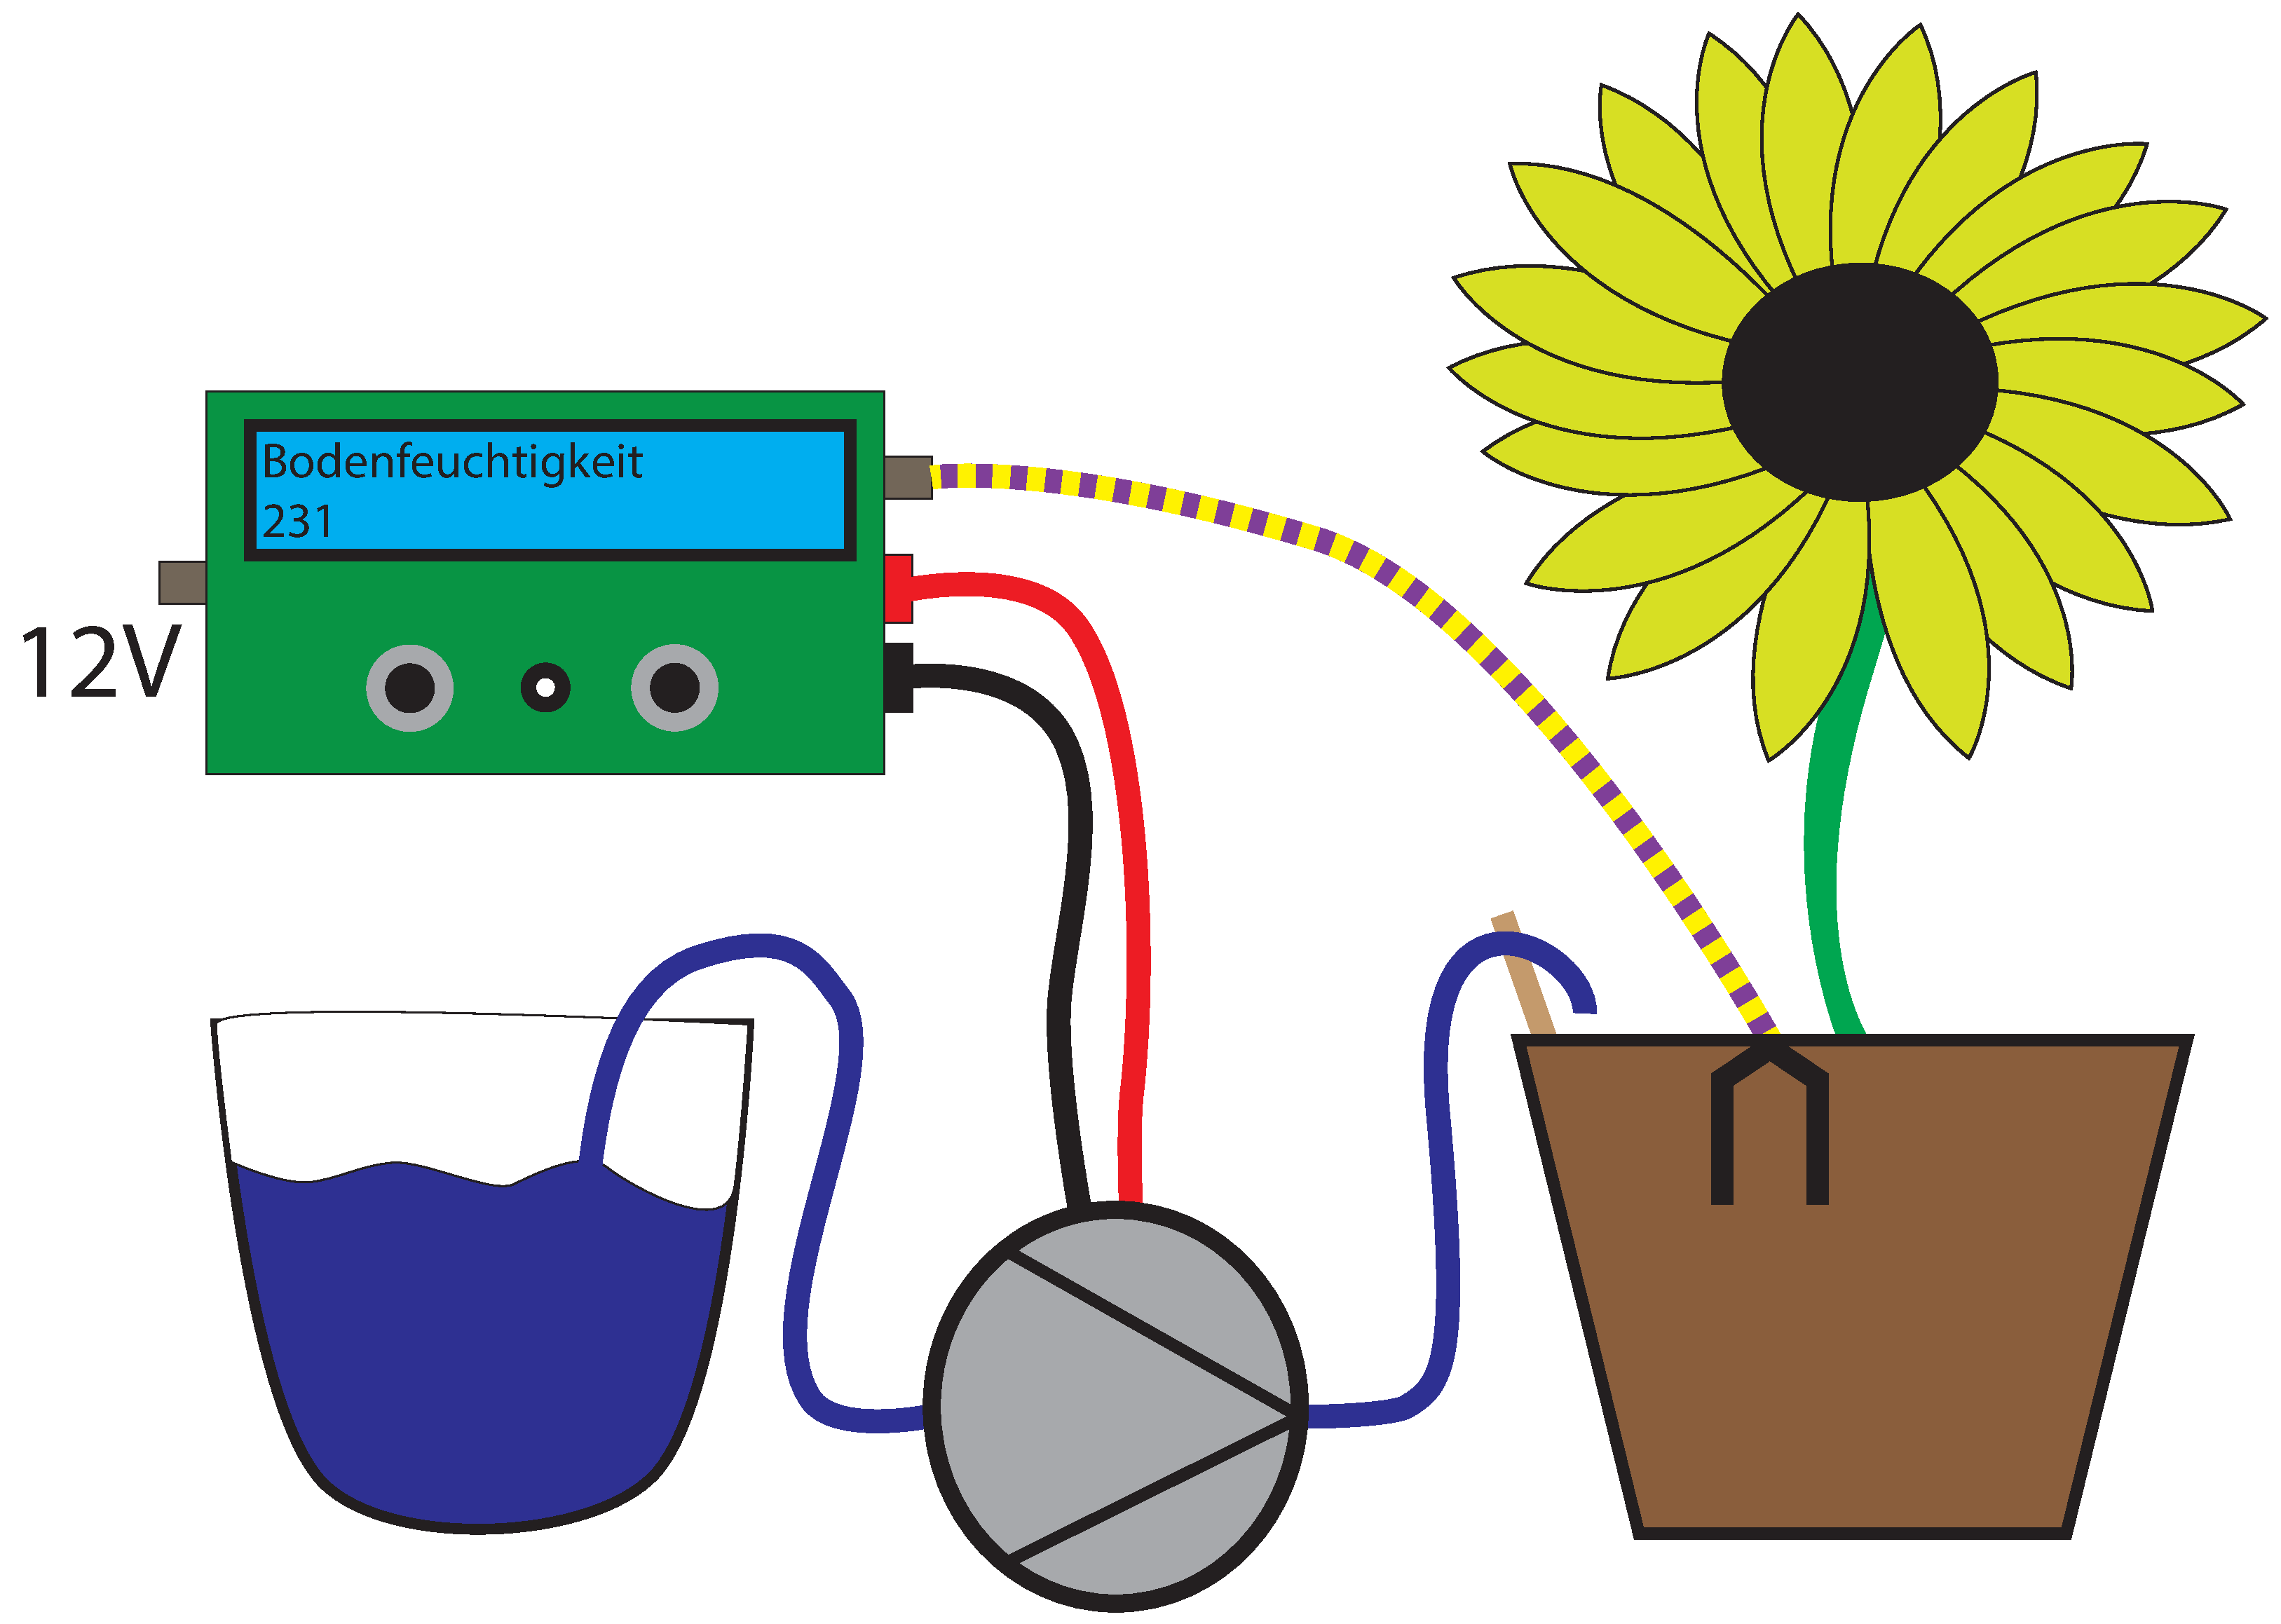
\includegraphics[width=0.9\linewidth]{bilder/Bild_Aufbau.eps}	
	\caption{Schematischer Aufbau der Gießanlage}
	\label{fig-SchemaAufbau}
	\end{figure}

\subsection{Wassertransport}
Um den Einsatzbereich so flexibel wie möglich zu gestalten, haben wir uns für ein Pumpensystem entschieden. 
Dadurch ist die Anordnung der Pflanze zum Wassertank nicht relevant. 
Der hiermit einhergehende, erhöhte Strombedarf ist zu verkraften, da das System nicht auf Batterien angewiesen ist.

Für den Wassertransport haben wir uns für eine Zahnradpumpe entschieden.
Die Zahnradpumpe gehört zur Gruppe der rotierenden Verdränger Pumpen\footnote{\href{http://www.ksb.com/Kreiselpumpenlexikon\_de/Pumpenlexikon/1563382/verdraengerpumpe.html}{www.ksb.com/Kreiselpumpenlexikon\_ \\ de/Pumpenlexikon/1563382/verdraengerpumpe.html}}.
Das Fördermedium wird hierbei zwischen zwei Zahnrädern in einem in sich geschlossenen Volumenbereich gefördert.
Die Bauweise dieser Pumpe ermöglicht zudem einen selbstsaugenden Betrieb. 
Dies bedeutet, dass diese Pumpe in der Lage ist Gase zu transportieren und somit einen Unterdruck in der Zuleitung zu erzeugen, der ausreicht um das Fördermedium (in unserem Fall Wasser) anzusaugen. 
Diese Eigenschaft war schlussendlich ausschlaggebend, dass sich die Zahnradpumpe gegenüber den anderen Lösungen durchgesetzt hat.
Als Alternativen wurden Ventile und Kreiselpumpen angedacht.
Die Kreiselpumpe konnte sich trotz dem geringeren Stromverbrauch und geringerem Geräuschpegel nicht durchsetzen. 
Das Ventil benötigt den geringsten Strom und ist sehr leise, jedoch ist es auf gespeicherte Energie angewiesen sind.  
Entweder durch Druck im Wassertank oder durch Erhöhung des Tankes über den Ausfluss. 
Auf Grund der Wahl der Zahnradpumpe kann ein 4\,mm Schlauch zur Förderung des Wassers genutzt werden, der nahezu beliebig verlegt werden kann.  
Ebenso ist der Wassertank frei wählbar. Für das Testsystem haben wir eine 1,5\,Liter Flasche verwendet. Im Dauerbetrieb wird ein fünf-Liter"~Weinballon verwendet. 
An der Pflanze wird der Schlauch mit einem durchbohrten Kantholz in der Pflanzenerde befestigt.

	
\begin{table}
	\centering
		\onehalfspacing
	\footnotesize
	\caption{Vergleich Wasserpumpen und Ventil}
	\label{Vergleich zwischen Wasserpumpen und Ventil}
		\begin{tabular}{|l|lll|}
		\hline
		\textit{Eigenschaft} & \textit{Zahnradpumpe} & \textit{Kreiselpumpe} & \textit{Ventil} \\
		\hline
		Selbstsaugend	&ja	&nein &nein\\		
		Lautstärke		&sehr laut	&mittel laut	&leises Klacken\\
		Stromverbauch	&@12V 2,8A	&@12V 0,6A	&@12V 80mA\\
		Förderleistung	&gering		&groß		&keine eigene\\
		Preis			&2,95 \euro	& 2,95 \euro	&	4,95 \euro\\
		\hline		
		\end{tabular}
		
\end{table}	
	
	

\subsection{Gehäuse}
	Das Gehäuse, wie es in Abbildung \ref{fig-Gehäuse} zu sehen ist, wurde so konzipiert, dass es möglichst klein ist aber dennoch genügend Platz für die Elektronik bietet.
	Im Gehäuse verbaut sind:
\begin{itemize}
	\item ein LCD-Display zur Anzeige der Gießparameter (aktuelle Feuchtigkeit, Gießintervall, \dots)
	\item zwei Taster zur Steuerung der Displayanzeige und zum manuellen Gießen
	\item der Photowiderstand zur Messung der Helligkeit (platziert zwischen den Tastern)
	\item Stromschluss auf der linken Seite
	\item Ausgänge für die Pumpe und den Feuchtigkeitssensor auf der rechten Seite

\end{itemize}	

	\begin{figure}[!h]
	\centering
	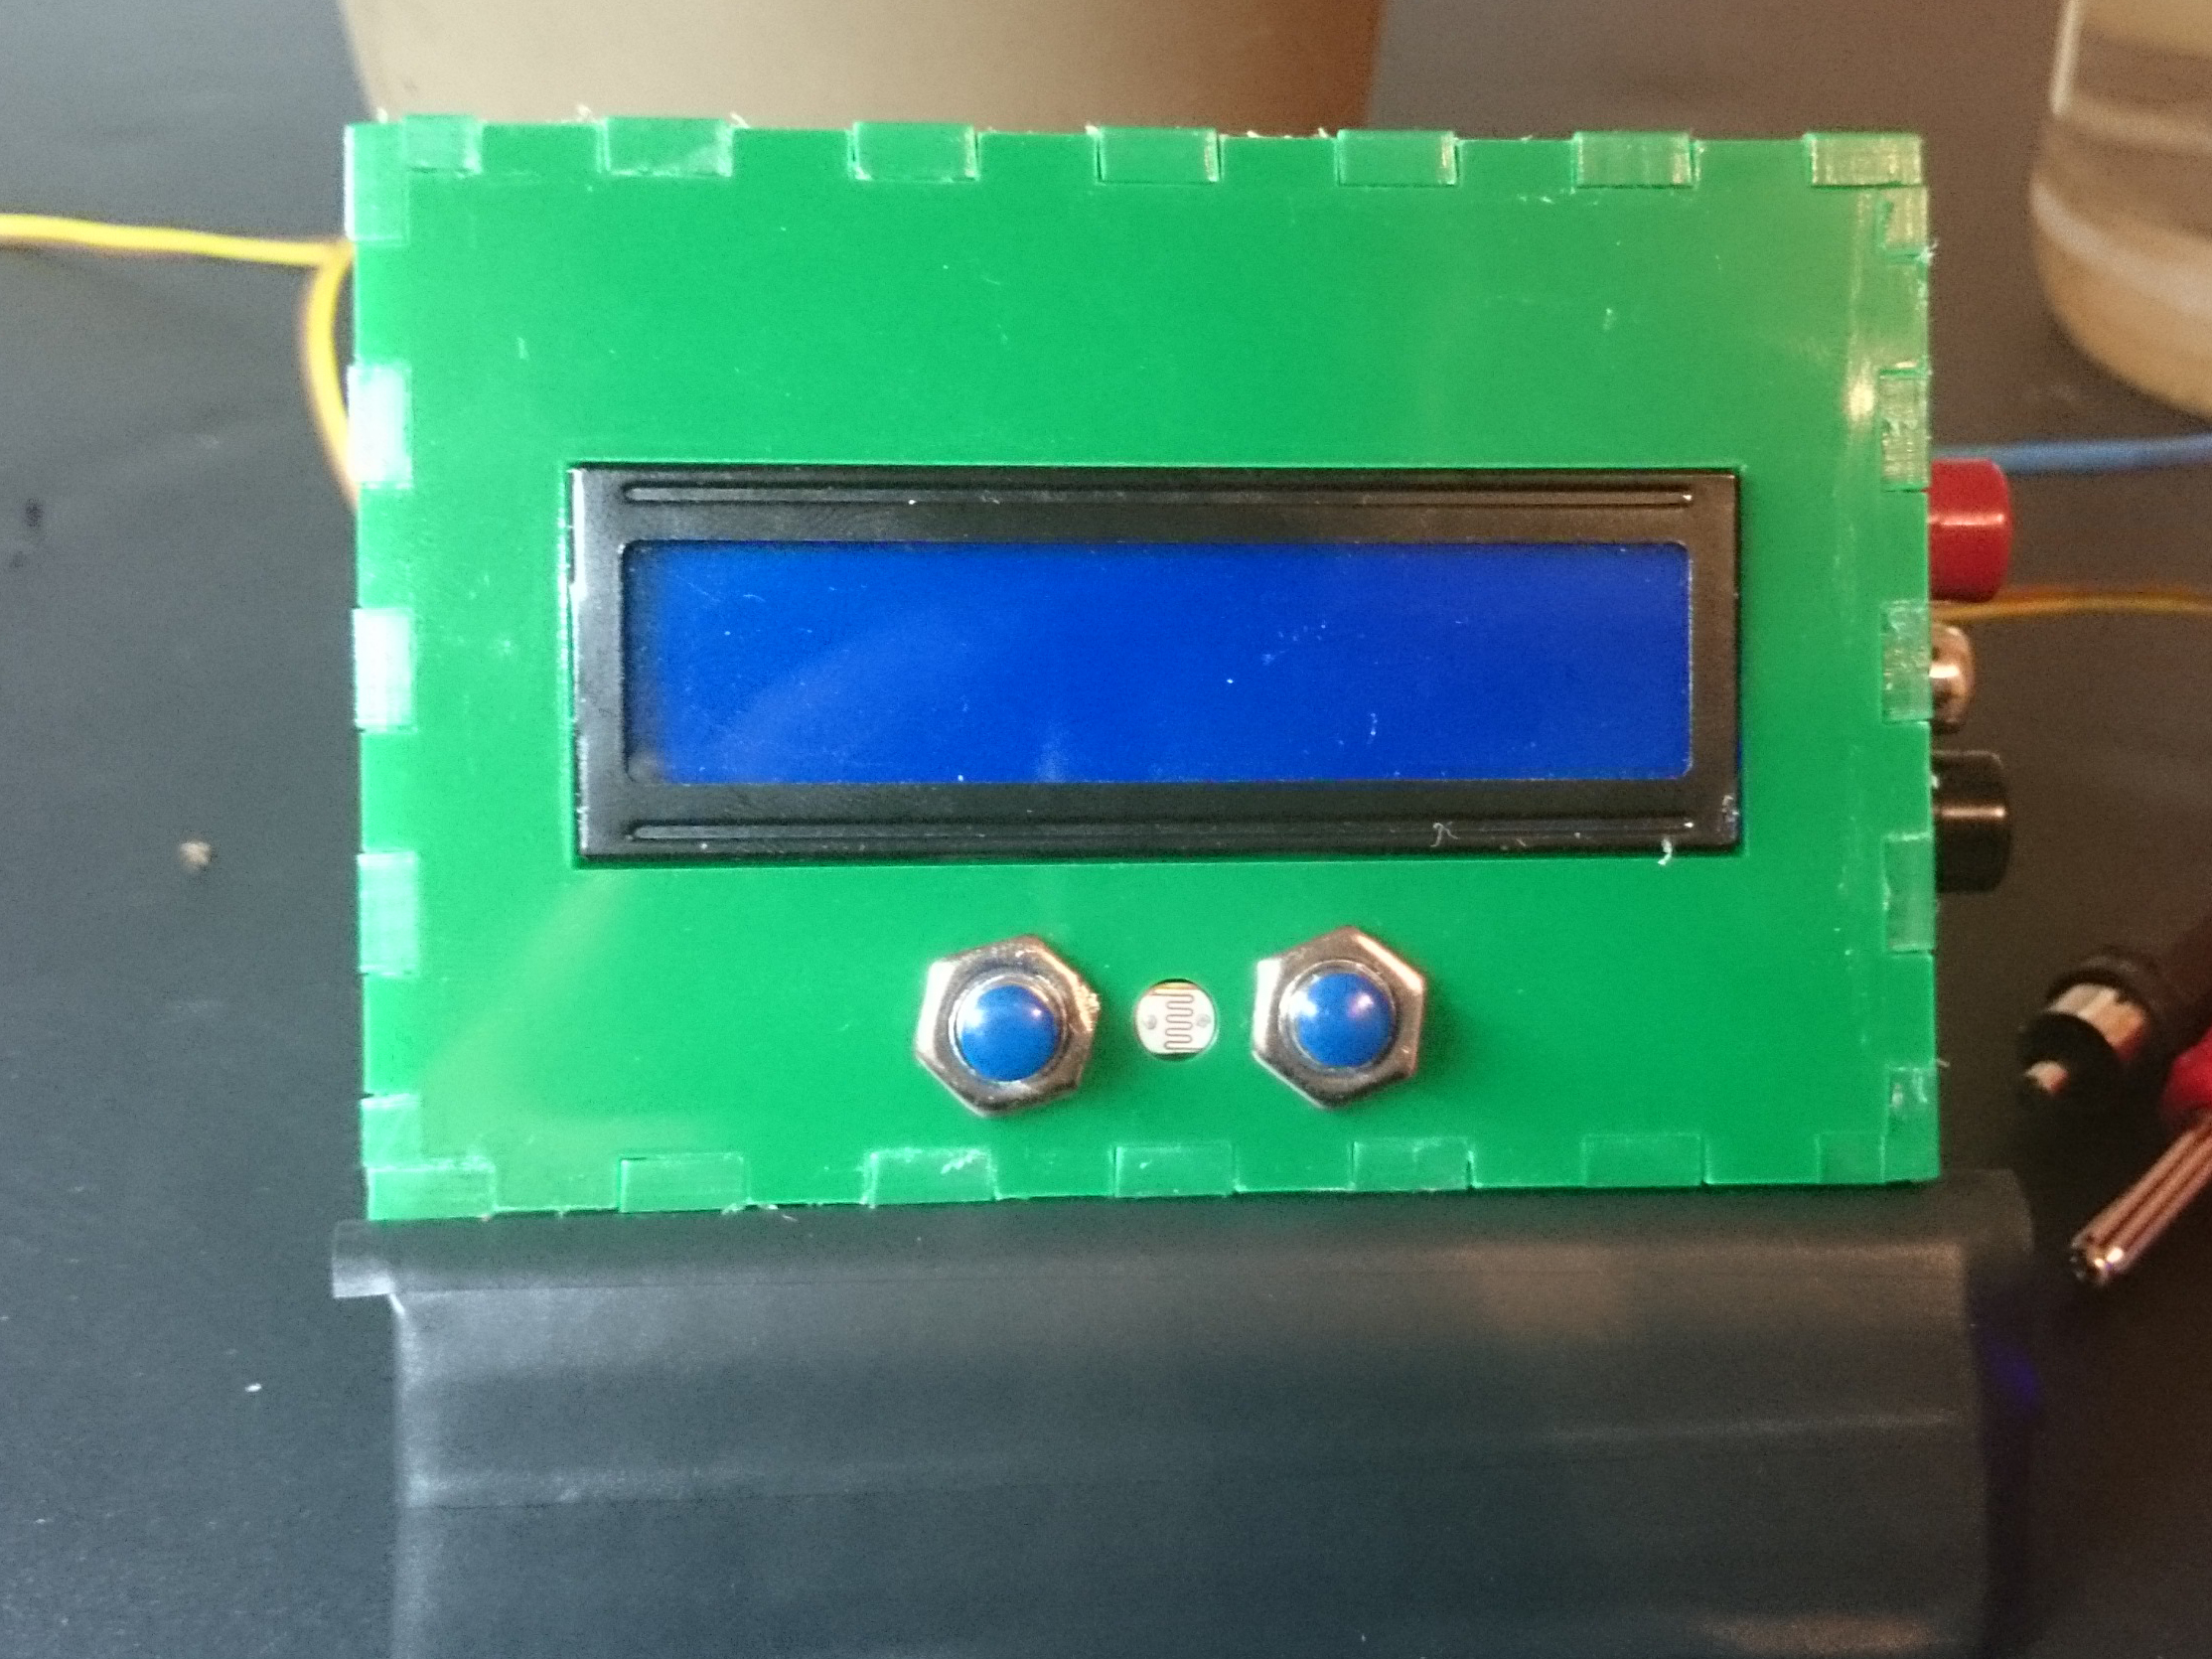
\includegraphics[width=0.9\linewidth]{bilder/_boxFron1.jpg}	
	\caption{Gehäuse Frontansicht}
	\label{fig-Gehäuse}
	\end{figure}
	
Das Gehäuse wurde in FabLab Erlangen mit einem Lasercutter gefertigt. 
Für das Design des Gehäuses wurde der BoxMaker\footnote{ \href{http://boxmaker.connectionlab.org/}{http://boxmaker.connectionlab.org/}} verwendet. 
Das Gehäuse besteht aus grünen 3\,mm dicken Acrylglas.
	
\subsection{Elektronik}
Im folgenden wird der Aufbau der Version~1.0 der \emph{Arduino"~Variante} vorgestellt. 
Während des Aufbaus -- vor allem aber während der Testphase -- sind Probleme aufgetreten, die dazu geführt haben, dass eine neue Version~1.1 erstellt werden musste. 
Diese neue Version ist jedoch aus zeitlichen Gründen noch nicht komplett aufgebaut. 
Ein neues Layout wurde erstellt und die Software ist so angepasst worden, dass diese ohne größere Änderungen übernommen werden kann. 
Daher wird im folgenden die Funktionsweise auf Basis der Version~1.0 erläutert, an gegebener Stelle wird auf die Anpassungen eingegangen, die bereits umgesetzt wurden bzw. noch in Planung sind. 

\begin{figure}[!h]
	\centering
	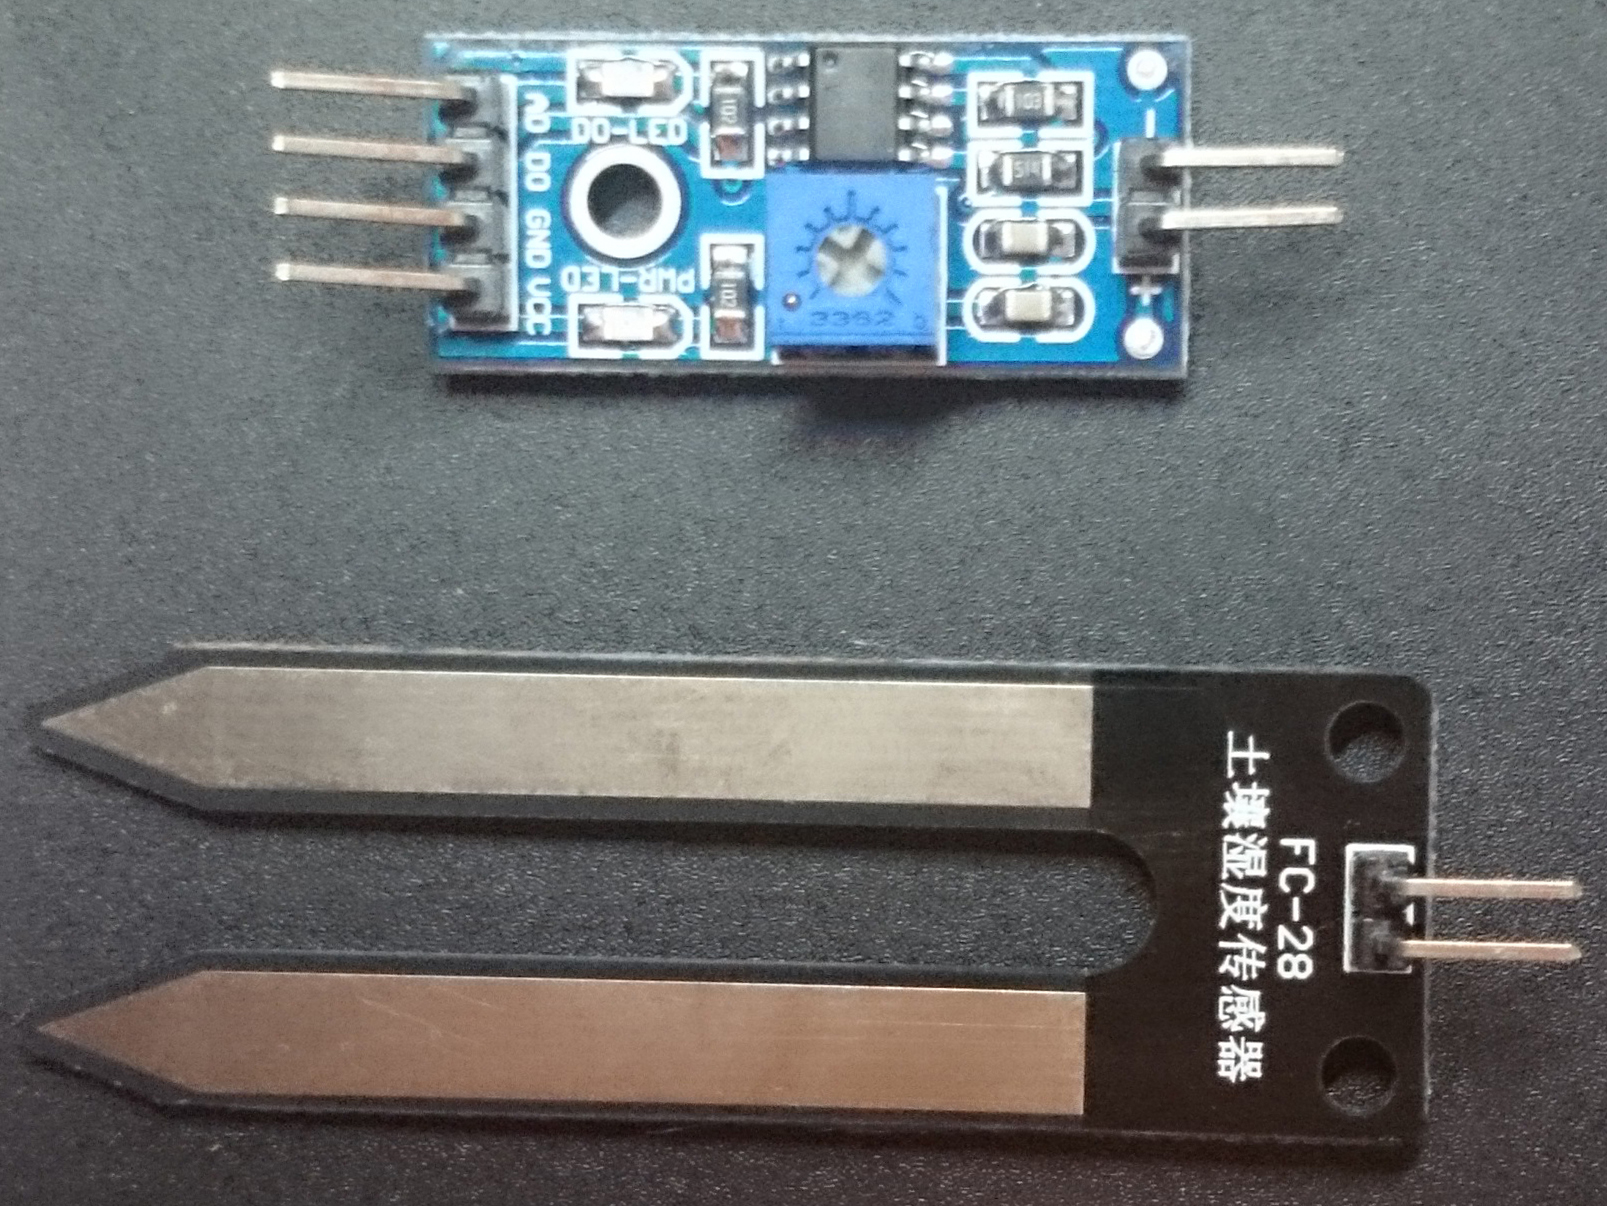
\includegraphics[width=0.9\linewidth]{bilder/_feuchteSensor1.jpg}
	\caption{Feuchtigkeitssensor mit Vorschaltung}
	\label{fig-SensorVorschaltung}
\end{figure}
			
\subsubsection{Sensorik} \label{sensorik}
Für den Helligkeitssensor wird ein einfacher Photowiderstand verwendet, der über einen Spannungsteiler an einem der analogen Pins des Arduino"~Bords angeschlossen ist. Der Pin verfügt über einen 10\,Bit"~AD Konverter und gibt demnach einen Integerwert von 
0\,-\,1023 zurück.
Der Bodenfeuchtigkeitssensor bestimmt den Wassergehalt des Bodens über eine Widerstandsmessung zwischen den zwei Zinken der Messgabel. 
Je mehr Wasser im Erdreich vorhanden ist, desto kleiner ist der gemessene Widerstand.


Der Feuchtigkeitssensor benötigt keine weiteren Schaltelemente, da er über eine eine Vorschaltung verfügt in der bereits ein Spannungsteiler integriert ist. 
Abbildung \ref{fig-SensorVorschaltung} zeigt den verwendeten Sensor und die Vorschaltung. 

Es ist möglich sowohl den analogen Wert als auch ein digitales Signal auszuwerten.
Das digitale Signal liefert einen Null"-wert solange ein Grenzwiderstand nicht überschritten wird. 
Über ein  Potentiometer (siehe Abbildung \ref{fig-SensorVorschaltung}) lässt sich diese Schaltwert einstellen. 
Wegen des schlechten Zugangs zum Potentiometer im eingebautem Zustand wird der digitale Output nicht verwendet, sondern der analoge Messwert selbst ausgewertet und mit einer Variablen im Mikrocontroller abgeglichen.

\begin{figure}[!b]
	\centering
	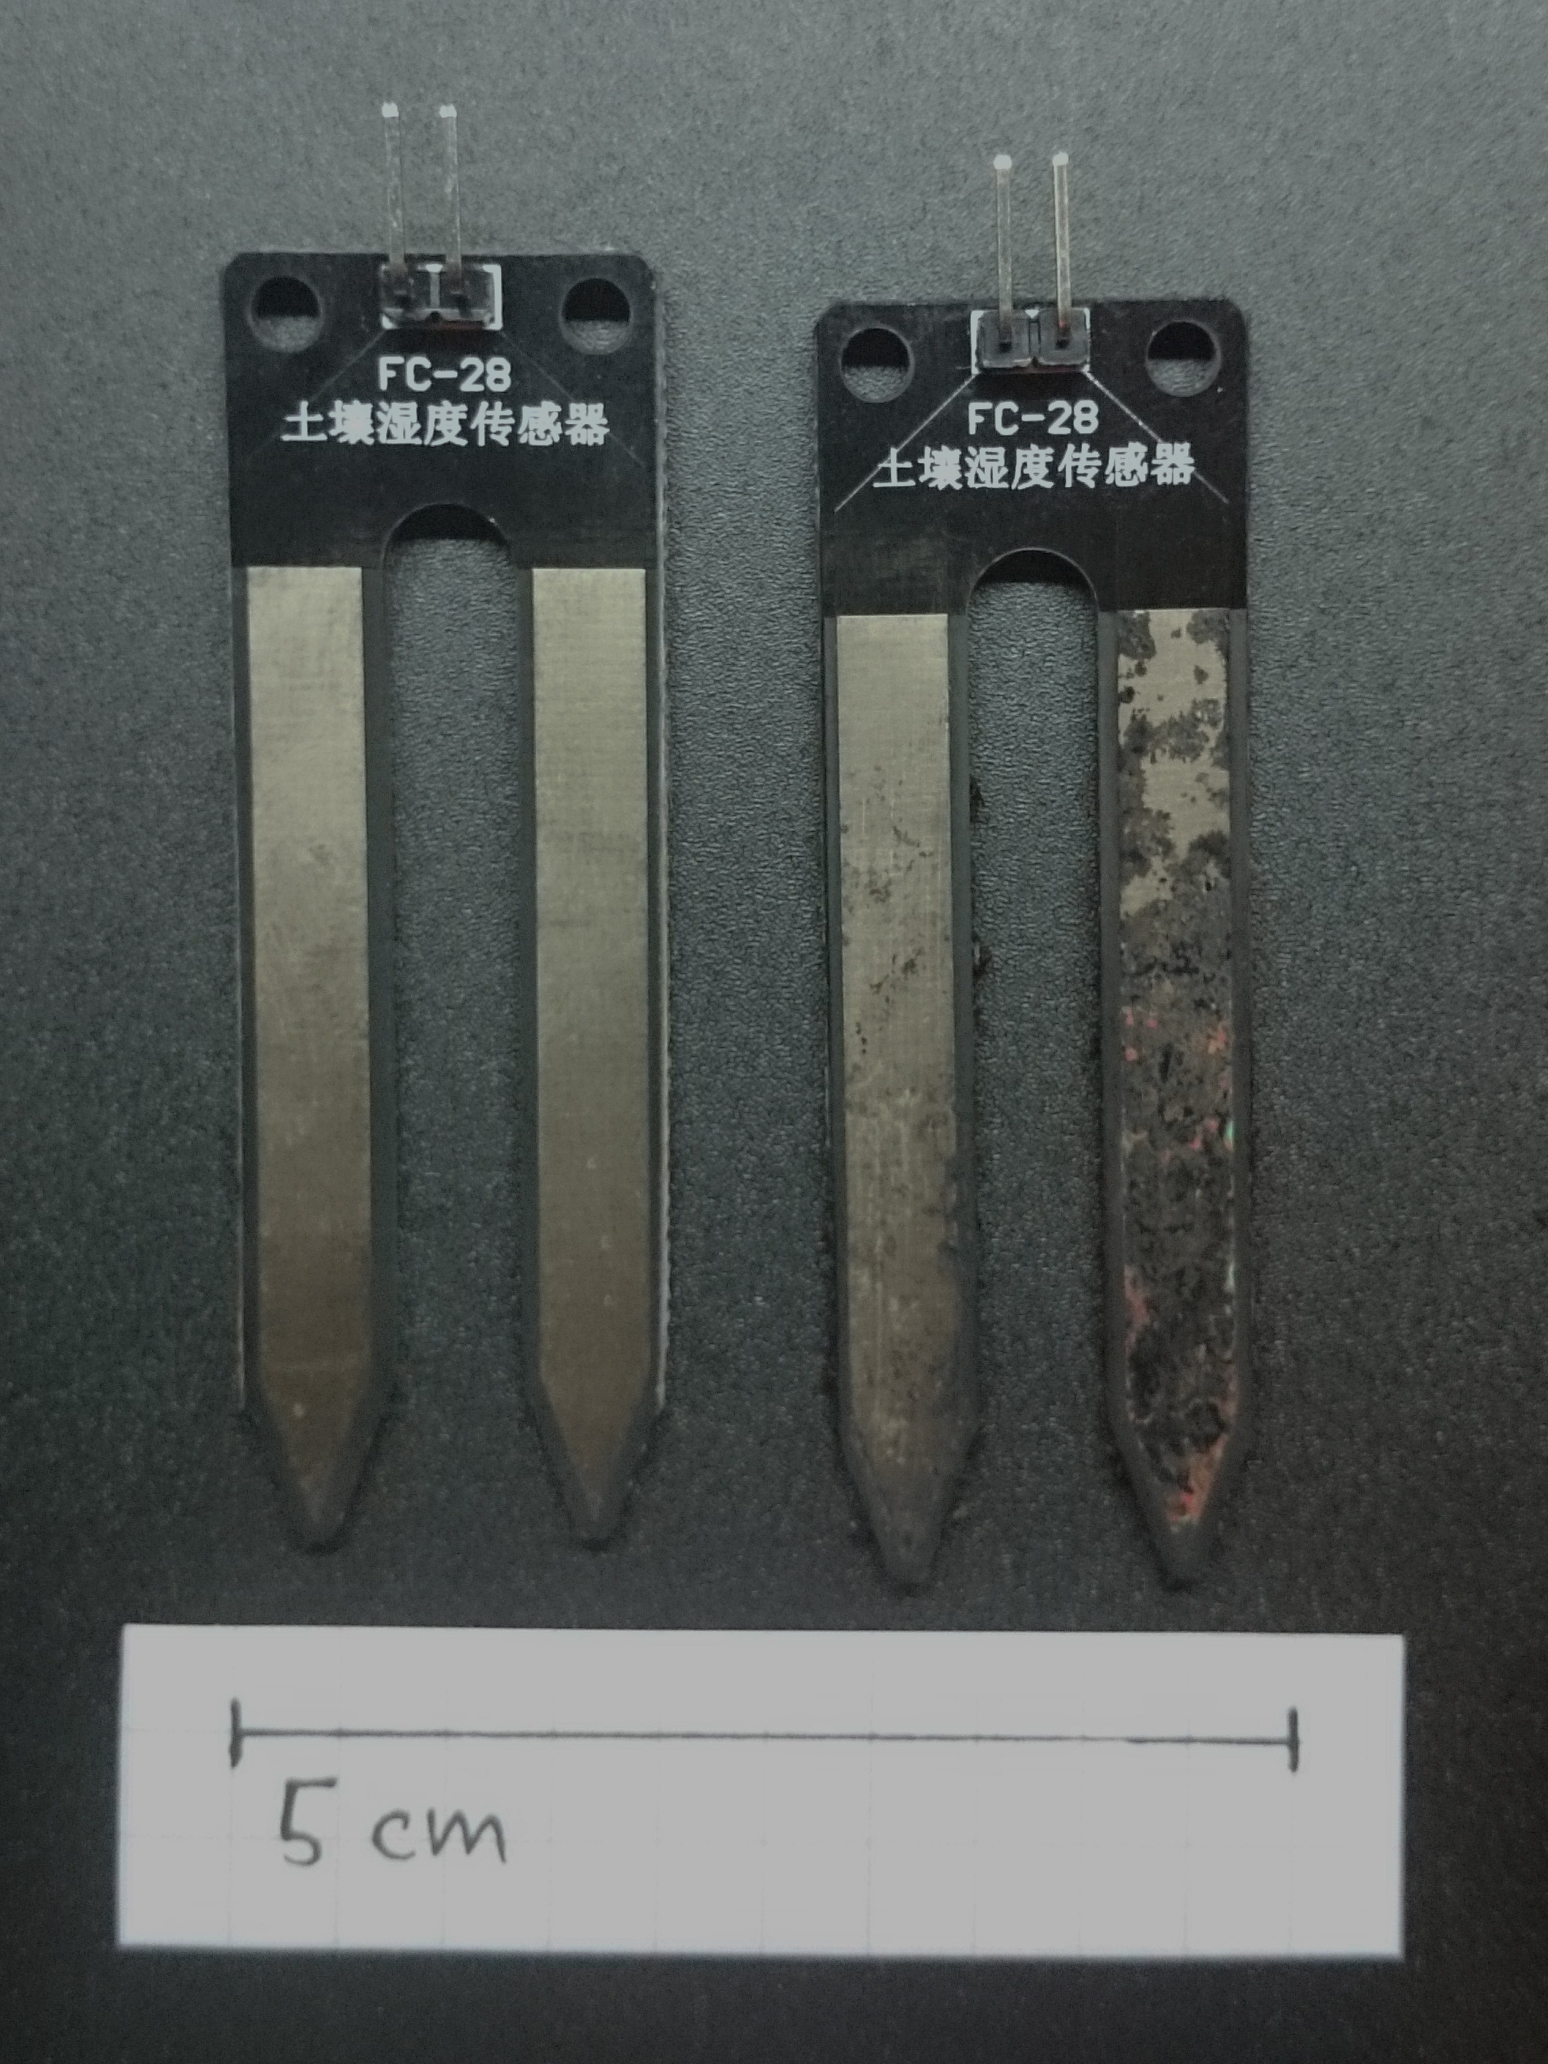
\includegraphics[width=0.9\linewidth]{bilder/_fechtesensorVergleich0.jpg}
	\caption{Vergleich neuer Sensor und Sernsor mit 48h Dauerbetrieb}
	\label{fig-SensorVergleich}
\end{figure}

\emph{Anpassung zu Version~1.1:}
Leider zeigte sich, dass nach nur 48 Stunden durchgehendem Messens die Gabel erhebliche Korrosionsschäden aufweist, Abbildung \ref{fig-SensorVergleich} zeigt dies deutlich.
Die Vorschaltung sieht weder eine Abschaltung des Messprozesses, noch eine Umpolung der Gabel-Polarität vor. 
Folglich muss die gesamte Vorschaltung stromlos geschaltet werden, um das Auflösen des Sensors möglichst zu verzögern. 
Hierfür haben wir für die Version~1.1 eine Transistorschaltung für den Sensor eingefügt. 
Über diese Schaltung wird die Vorschaltung des Feuchtigkeitssensor stromlos geschaltet und der Sensor nur für eine Messung mit Strom versorgt. 
Eine Umpolung der Messgabel ist hiermit nicht möglich. Dies kann jedoch relativ einfach gelöst werden, indem der Sensor alle paar Wochen \emph{manuell} umgepolt wird. 
Hierfür muss lediglich die Messgabel vom Verbindungskabel abgesteckt, um \begin{math}180^{\circ}\end{math} gedreht und wieder verbunden werden.



\begin{figure}[h]
	\centering
	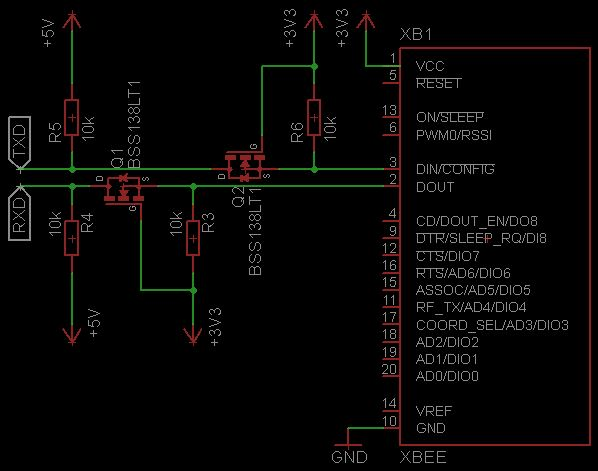
\includegraphics[width=0.9\linewidth]{bilder/v1SchaltplanXbee.jpg}
	\caption{Pegelwandler mit Small-Signal-Transistor BSS138W }
	\label{fig-Pegel}
\end{figure}

\begin{figure*}[th]
	\centering
	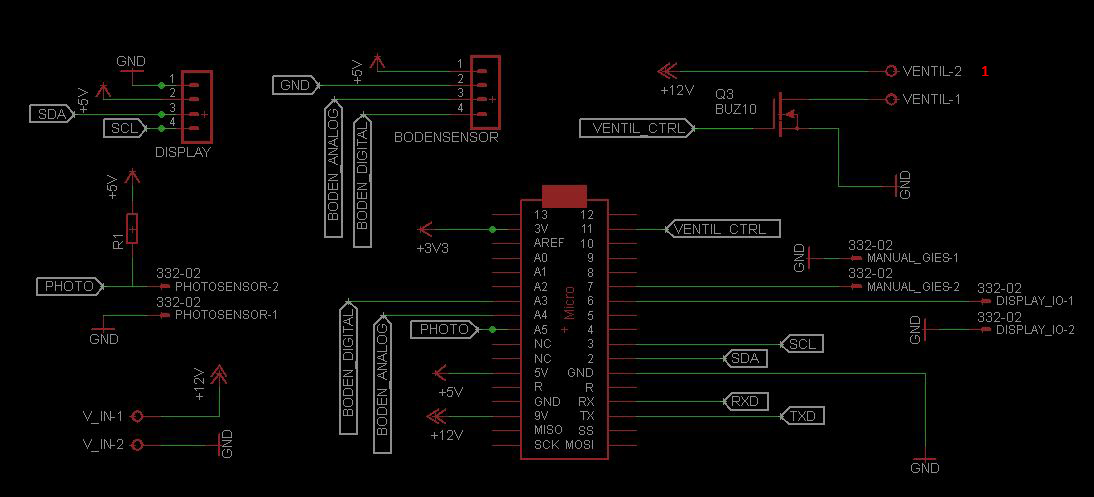
\includegraphics[width=0.85\linewidth]{bilder/v1SchaltplanMicro0.JPG}
	\caption{Schaltpaln V1.0 mit Arduino Micro}
	\label{fig-Schaltplanv1.0}
\end{figure*}

\subsubsection{Kommunikation}
Ziel der Kommunikation ist es, das Gießsystem im laufenden Betrieb kalibrieren zu können. 
Wir haben uns für eine drahtlose Kommunikation auf Basis des XBee Standard entschieden. 
Das XBee Modul wurde direkt, d.h. ohne Verwendung eines \emph{Arduino XBEE"~Shields} mit dem Arduino verbunden. 
Hierfür war es notwendig eine Pegelwandlung von 5\,V auf 3,3\,V vorzunehmen, da die Logik-Pins des XBee"~Moduls nicht mit 5\,V des Arduinos betrieben werden können. 
%%%%%%
Abbildung \ref{fig-Pegel} zeigt die Umsetzung der Pegelschaltung. Die Lables \emph{TXD} und \emph{RXD} repräsentieren die jeweiligen Anschlüsse am Arduino Micro. In dieser Schaltung lassen sich drei Zustände erkennen\footnote{http://www.adafruit.com/datasheets/an97055.pdf; Seite 10f}:
\begin{itemize}
\item Wird keiner der beiden Seiten (Mikrocontroller bzw. XBee) auf GND gezogen, so werden die Eingänge durch ihre Pull-Up 	Widerstände auf 5\,V bzw. 3,3\,V gezogen.
Dadurch ist das Spannungsgefälle \emph{Gate"~zu"~Source} gleich Null, da an beiden Anschlüssen 3,3\,V anliegen. Der Transistor ist nicht leitend.
\item Wird am XBee (DOUT) ein LOW Signal angelegt, so steigt das Spannungsfälle \emph{Gate"~zu"~Source} an und der Transistor wird leitfähig, was dazu führt das auch die Pins am Mikrocontroller(RXD) auf LOW gezogen werden.
\item Wird hingen auf der Seite des Mikrocontroller (TXD) ein LOW Signal angelegt, so wird über die Diode im Transistor das Spannungspotenzial der Source solange reduziert, bis das Spannungsgefälle \emph{Gate"~zu"~Source} groß genug wird, damit der Transistor leitfähig wird. Sobald dieser Grenzwert überschritten wird, wird auch DIN am Xbee auf LOW gezogen.
\end{itemize}

Bei der Pegelschaltung ist uns in Version~1.0 ein Fehler unterlaufen, weswegen wir keine Verbindung mit ein Computer aufbauen konnten. Dieser Fehler ist für die Version~1.1 behoben.





		
Die zweite Schnittstelle zum Anwender ist das Display. 
Hier lässt sich über einen Taster die einzelnen Variablen mit ihren aktuellen Werten überprüfen. 
Bei dem Display handelt es sich um ein 2"~zeiliges LCD"~Display mit jeweils 16 Zeichen. 
Die Kommunikation zwischen Display und Mikrocontroller wird über eine I2C"~Schnittstelle bewerkstelligt. 
Hierfür haben wir die frei verfügbare \mbox{LiquidCrystal\_I2C} Libary von fderbrabander verwendet.\footnote{\href{https://github.com/fdebrabander/Arduino-LiquidCrystal-I2C-library}{https://github.com/fdebrabander/Arduino-LiquidCrystal-I2C-library}}


	
\subsubsection{Stromversorgung}

Eine Stromversorgung über USB ist nicht möglich, da die Pumpe unter Voll"-last 12\,V und 2,8\,A benötigt. 
Deswegen muss auf eine leistungsfähigere Energiequelle gesetzt werden.
Um den Strom der Pumpe zu begrenzen, wurde ein \begin{math}5~\Omega\end{math}\,Lastwiderstand in Reihe geschaltet.
Dies führt zu geringerer Leistungsaufnahme und einer deutlichen Geräusch"-minderung.
Die Ansteuerung der Pumpe über dem Mikrocontroller ist über eine Transistorschaltung gelöst (Ziffer 1 in Abbildung \ref{fig-Schaltplanv1.0}).
Es ist zu überlegen, den Transistor und den Mikrocontroller über eine Schutzdiode über die Anschlüsse \emph{VENTIL-1} und \emph{VENTIL-2} vor Überspannung zu schützen, die beim Abschalten der Pumpe auftreten können. 
 

\subsection{Programm}
	

	Die Aufgaben des Mikrocontrollers sind die folgenden:
		\begin{itemize}
			\item Messung der Feuchtigkeit
			\item Messung der Helligkeit
			\item Vergleich der Messwerte mit den festgelegten Grenzen
			\item Ansteuerung des Pumpensystems
			\item Ausgabe der wichtigen Variablen auf dem Display über Taster
			\item Manuelles Gießen über Taster
			\item Display Hintergrundbeleuchtung abschalten nach 60 Sekunden
			\item Übertragen/Empfangen von Einstellungen über XBee Verbindung
		\end{itemize}
		
	

	
In Abbildung \ref{fig-AV_Ablaufplan} ist der Ablauf des Arudino"~Programms in der Loop"~Methode zu sehen.
Wie in Abschnitt \ref{sensorik} beschrieben, führt eine dauerhafte Messung der Bodenfeuchtigkeit zu einer schnellen Zersetzung des Sensors.
Aus diesem Grund wird die Messung nur einmal in einem Intervall von ca.~4~Stunden durchgeführt. Für die Intervall"~Abfrage in der Methode \emph{messung()} wird die Funktion \emph{millis()} verwendet. Diese Funktion gibt einen unsigned Long Wert zurück, welcher der Laufzeit des Arduino in Millisekunden entspricht. Nach ungefähr 49 Tagen wird der Counter einen Überlauf erzeugen und beginnt von vorne zu zählen. Damit dieser Überlauf keine Auswirkungen auf das Gießsystem hat, wird die Abfrage des Messintervalls wie folgt ausgeführt.

\begin{lstlisting}[basicstyle=\small]
if ((millis()-prevMessung) >= messInterval)
{
 aktFeuchtigkeit = analogRead(MOISTURE_A);
 aktHelligkeit = analogRead(PHOTO_PIN);
 neueMesswerte = true; 
 prevMessung = millis();
}
\end{lstlisting}

Beim ersten Durchlauf, also direkt nach dem Anschalten des Mikrocontrollers, wird die If"~Bedingung immer als \emph{wahr} evaluiert und eine Messung wird durchgeführt. In die Variable \emph{prevMessung} wird die aktuelle Zeit eingestellt. Dadurch wird die If"~Abfrage erst dann wieder \emph{wahr}, wenn die Zeit \emph{messInterval} abgelaufen ist. Auch bei einem Überlauf der Funktion \emph{millis()} wird diese Abfrage ein korrektes Ergebnis liefen, da die Funktion \emph{millis()} einen unsigned Long zurück gibt. Bei allen Intervall"~bezogenen Abfragen im Programmcode wird dieses Vorgehen verwendet. 

Anpassung zu Version~1.1: In dieser Abfrage wird die Messung lediglich alle 4 Stunden durchgeführt. Für die Version 1.1 muss in diesem Programmabschnitt noch das An- und Abschalten des Feuchtigkeitssensors durchgeführt werden. Außerdem ist es, um Messfehler zu vermeiden, sinnvoll, nach dem Anschalten des Sensors kurz zu warten bevor eine Messung durchgeführt wird.

Unabhängig davon, ob eine Messung ausgeführt wurde oder nicht, wird im Anschluss überprüft, ob der Mode"~Taster betätigt wurde. Wie in Abbildung \ref{fig-Schaltplanv1.0} zu sehen ist, wurden die Taster nicht über einen Kondensator entprellt, sondern per Software. Hierfür haben wir die Bounce2 Libary verwendet\footnote{http://playground.arduino.cc/Code/Bounce}. Wurde ein Knopfdruck registriert, so wird die Variable \emph{Mode} inkrementell erhört. Über die Modulberechnung wird sichergestellt, dass die Variable immer das Intervall von \emph{0~bis~ANZAHL\_MODE} durchläuft. Der Zweite Taster dient zum manuellen Gießen der Pflanze. Solange der Taster gedrückt ist, wird die Pumpe angesteuert und es wird gegossen. 

\begin{lstlisting}[basicstyle=\small]

mode = (mode + 1) % ANZAHL_MODE;

\end{lstlisting}

Als nächstes wird überprüft, ob ein neuer Messwert vorhanden ist.
Dies wird über die Variable \emph{neueMesswerte} bewerkstelligt. Diese Variable wird gesetzt, sobald eine Messung durchgeführt wurde (siehe oben).
Ist das nicht der Fall, so wird wie in Abbildung \ref{fig-AV_Ablaufplan} zu sehen ist, die Methode \emph{Gießen()} mit dem Parameter \emph{false} aufgerufen und die Variable \emph{neuerMesswert} auf \emph{false} gesetzt.
Damit wird verhindert, dass auf Grundlage des selben Messwertes erneut eine Entscheidung getroffen wird.
Sagt der Messwert hingegen aus, dass gegossen werden muss aber der Helligkeitssensor verhindert ein Gießen, dann wird die Variable \emph{neuerMesswert} nicht zurückgesetzt.
Der Aktuelle Messwert wird demnach solange abgeglichen, bis es hell genug ist, damit gegossen werden kann.

Abschließend wird in der Logikkette eine Methode zum Anzeigen der Messwerte auf dem LCD"~Display aufgerufen. Diese zeigt die Einstellung an, welche mit der Mode"~Variable korrespondiert ( 1 = akt. Bodenfeuchtigkeit, 2 = akt.  Helligkeit, \dots). 
Die Bausteine \emph{DatenEmpfang()} und \emph{DatenSenden()} sind in Version~1.0 noch nicht implementiert, da ein Fehler im Schaltkreis der Kommunikationsschnittstelle eine Kommunikation nicht möglich macht. Diese werden jedoch in Version~1.1 abgebildet.

\begin{figure}[h]
	\centering
	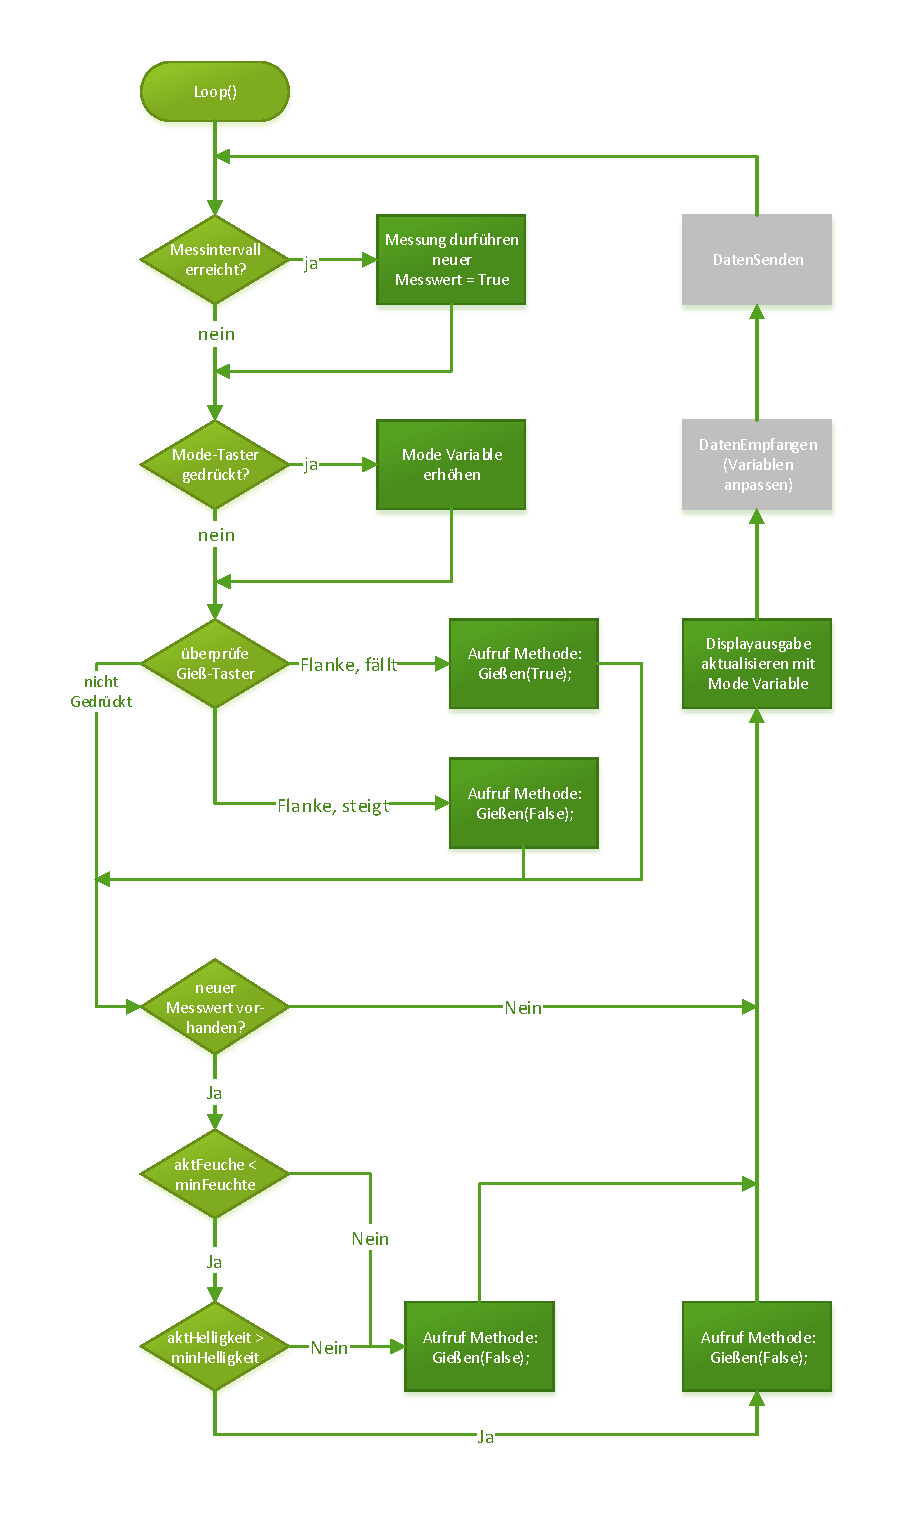
\includegraphics[width=\linewidth]{diagramme/AV_Ablaufdiagramm.pdf}
	\caption{Programmablauf der Arduino Version}
	\label{fig-AV_Ablaufplan}
\end{figure}
	
\subsection{Kostenplan}

 Durch die geringen Kosten pro Entwicklungsstufe hatten wir genügend Mittel um mehrere Iterationsstufen  zu durchlaufen.
 Dementsprechend benötigten wir für die gesamte Entwicklung etwas über einhundert Euro.
 Ein einzelnes Modul kann für etwa 45\,\euro\ nachgebaut werden. 
 Die Kosten setzen sich nach Tabelle\,\ref{Kosten für eine Giessanlage} zusammen.
 
 Nicht berücksichtigt sind das Wassergefäß, die zwei \begin{math}4mm\end{math}\,-Schlauch"-Stücke und die Befestigung in der Pflanze.
 Bei diesen handelt es sich um Reste oder Lagerfunde im Wert von unter 1\,\euro. 

 
\begin{table}[ht]
	\centering
	\onehalfspacing
	\footnotesize
	\caption{Kosten für eine Gießanlage}
	\label{Kosten für eine Giessanlage}
		\begin{tabular}{|l|ll|}
			\hline
\textit{Bauteil} & \textit{Kosten} & \textit{Bezugsquelle} \\
\hline
Arduino Nachbau & ca. 3 \euro & ebay \\
LCD-Display & ca. 5 \euro & ebay\\
Bodensensoren & ca. 2 \euro & ebay \\
Zahnradpumpe & 2,95 \euro & Pollin \\
XBee &  23,55 \euro & Reichelt \\
Hauptplatine & ca. 6 \euro & FabLAB \\
Gehäuse	& ca. 4 \euro & FabLAB \\

\hline
Gesamt: & ca 45 \euro & \\
\hline
\end{tabular}
\end{table}


%section

\section{Sparversion}
	Um Strom zu sparen, die Größe zu schrumpfen und Kosten günstiger zu werden, haben wir die \glqq Sparversion\grqq entwickelt.
	In dieser Variante der Gießanlage wurde die Anlage auf das wesentlichste beschränkt,das Gießen.
	Sie wurde so konzipiert, dass sie genau auf eine Pflanze zugeschnitten ist.
	Sie kann nur durch erneutes Programmieren auf andere Pflanzen und Böden angelernt werden. 	
	\subsection{Aufbau}
	In dieser Version wird auf das Display und die Kommunikation verzichtet.
	Dadurch wird viel der Verkabelung gespart, außerdem lässt sich die Hauptplatine deutlich kleiner gestalten.
	Dies führt zu weniger Platz"-bedarf des Systems und dazu das es in ein kleineres Gehäuse passt.
	\subsection{Elektronik}
	Durch das WEgfallen der XBee Platine und deren Beschaltung wird das 3,3\,V Netz nicht mehr benötigt.
	Die Größe der Hauptplatine  reduziert sich auf \begin{math} 55 mm \times 32 mm \end{math}.
	Dies entspricht weniger als der Hälfte der Fläche der Version 1.1 mit \begin{math} 56 mm \times 65 mm \end{math}.
	\subsection{Programmierung}
	Um weiter Stromsparen zu können wurde diese Version nicht mit Arduino, sondern mit C geschriebenen Programm programmiert.
	Dies ermöglicht die Ausnutzung der Sleep Modi und die Interrupts des ATMega328. 
	Dadurch befindet sich der \glqq Arduino Nano\grqq \ hauptsächlich im Schlafmodus und verbraucht deutlich weniger Energie.
	Die Gießeinstellungen müssen auf Grund der fehlenden Kommunikation und Eingabemöglichkeiten über die Programmierung festgelegt werden.
	\subsubsection{Programmierwerkzeuge}
	Durch das Wegfallen der Arduino Bootloaders, kann die Hardware nicht mehr per USB programmiert werden. 
	Mit Hilfe des AVRISP mkII \footnote{\href{http://www.atmel.com/tools/avrispmkii.aspx}{www.atmel.com/tools/avrispmkii.aspx}} kann der Mikrocontroller über die ISP-Schnittstelle mit den Binärcode beschrieben werden. 

	\subsubsection{Logik}
		\begin{figure}[!h]
	\centering
	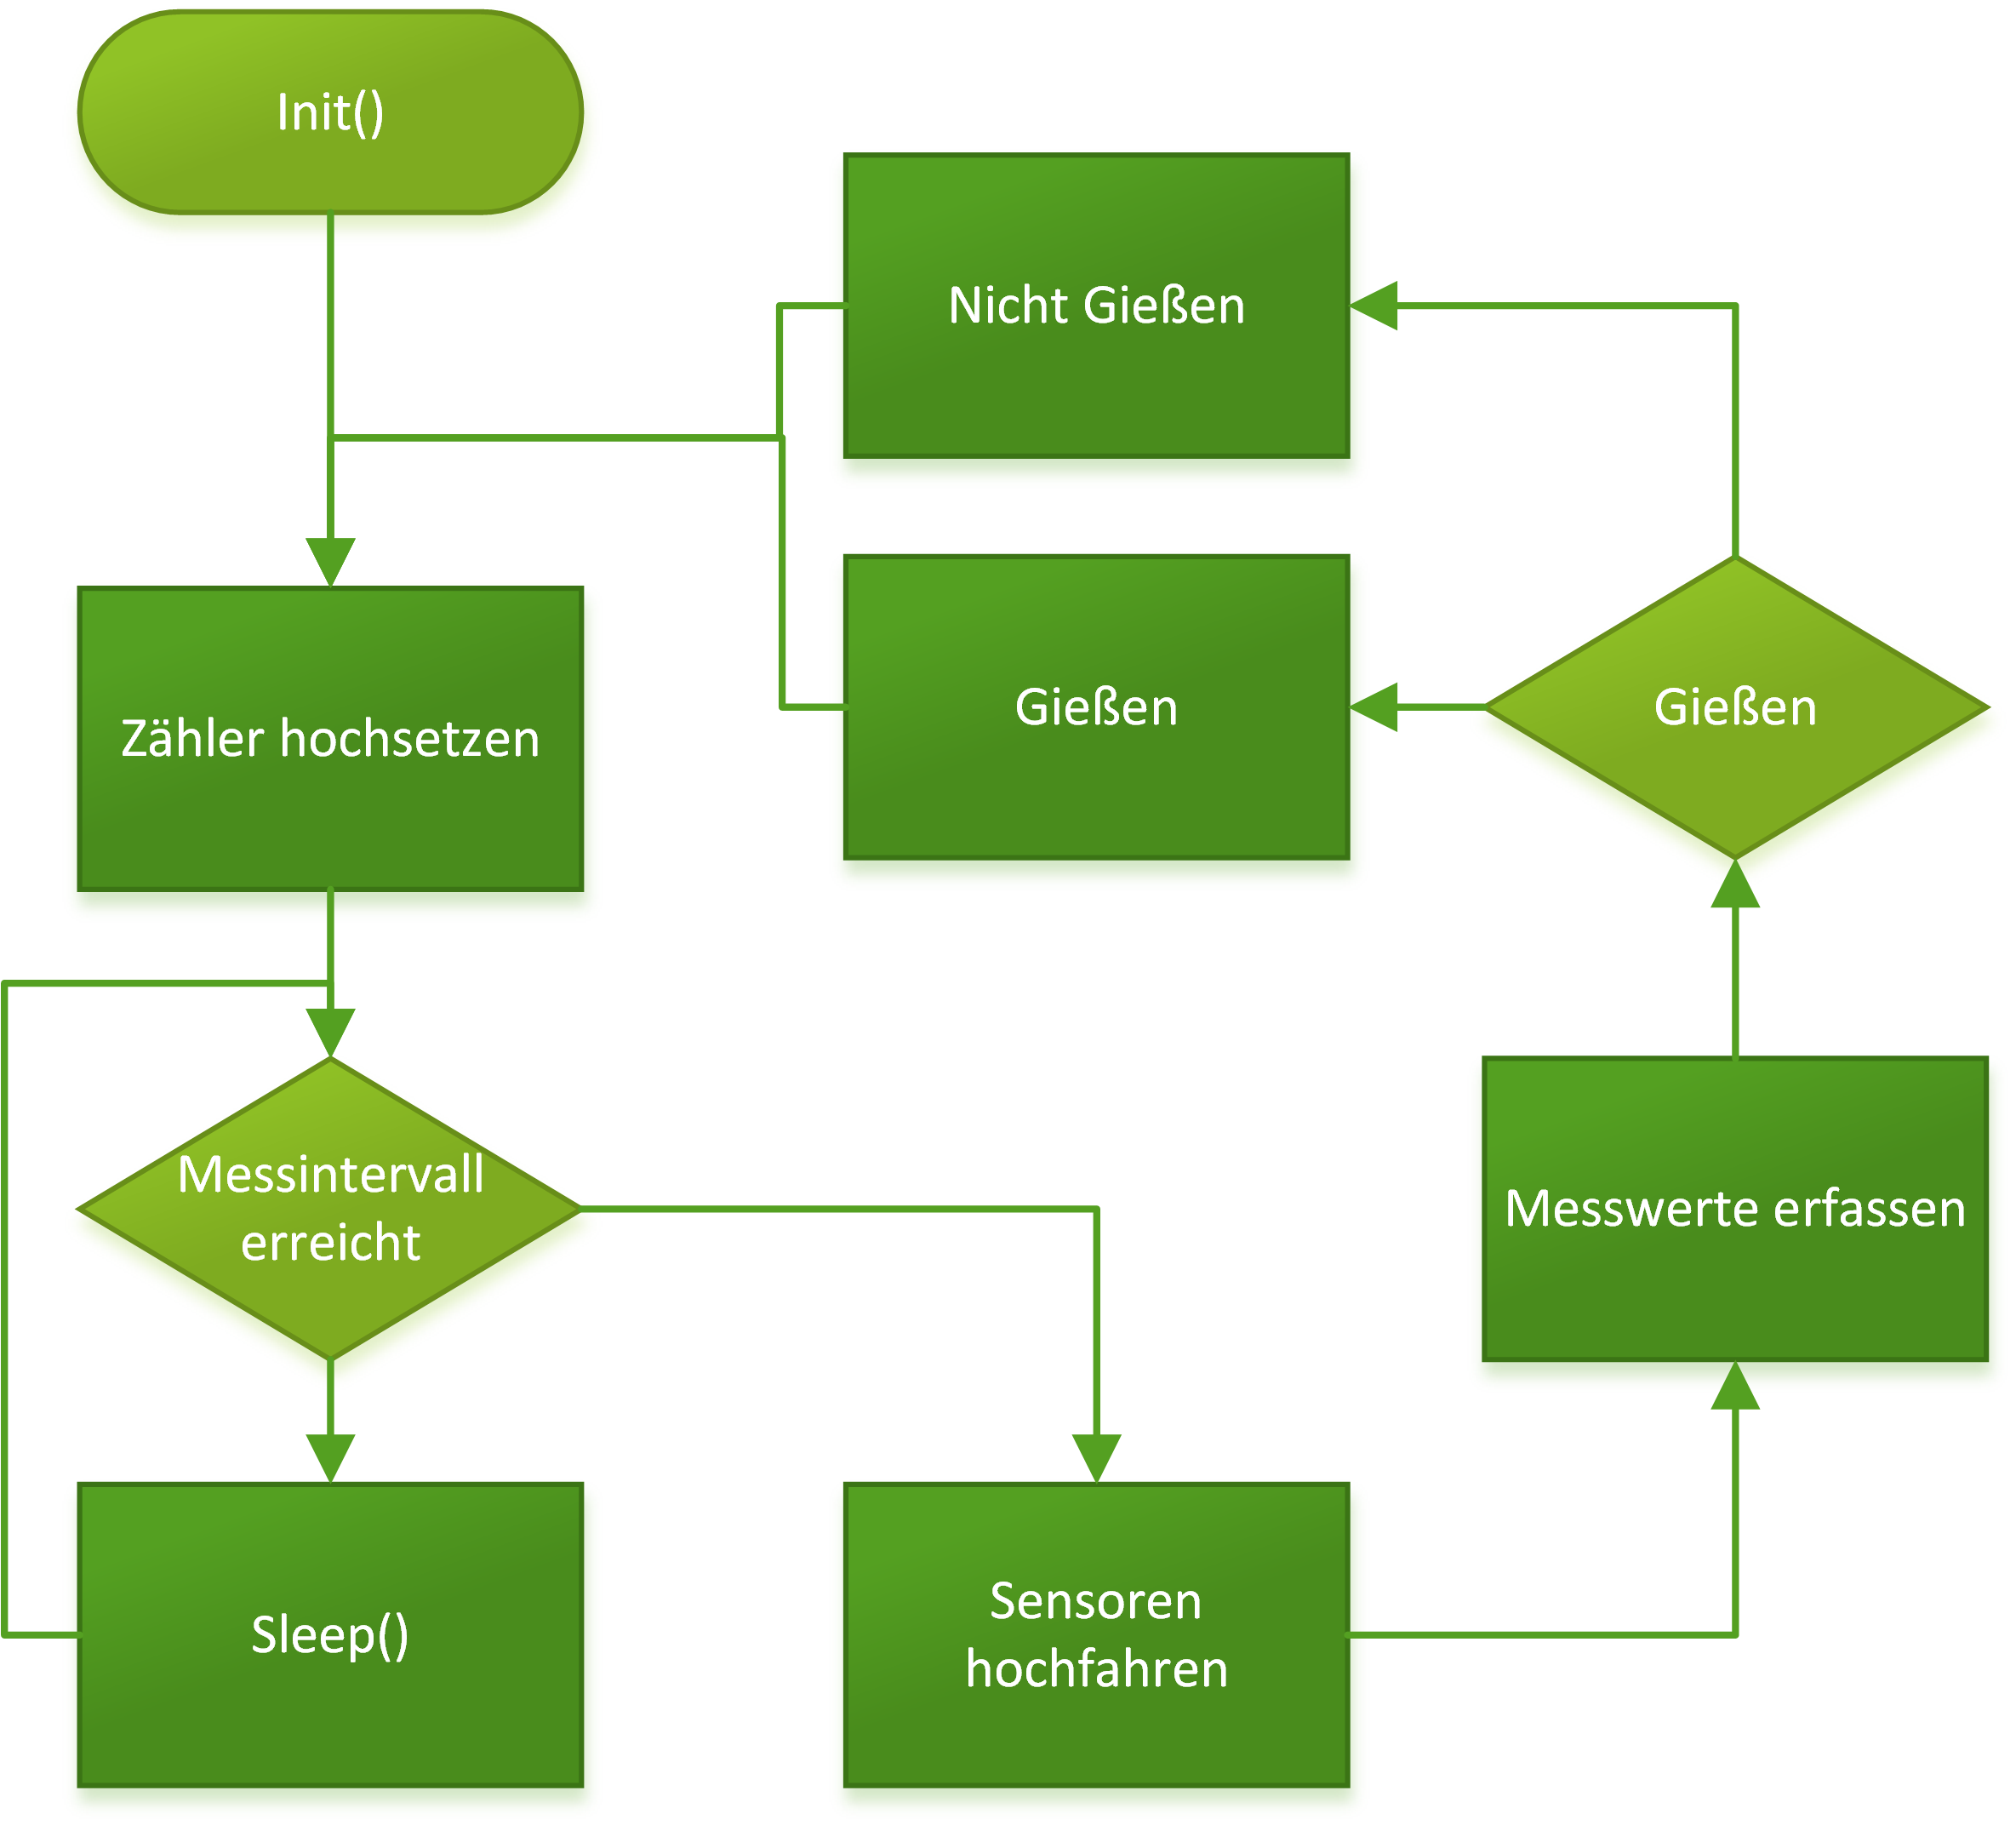
\includegraphics[width=0.8\linewidth]{Diagramme/SV_Ablaufdiagramm.png}
	\caption{Ablaufplan des Programms der Sparversion}
	\label{fig-SV_Ablaufplan}
\end{figure}

	Der Ablaufplan (Abbildung \ref{fig-SV_Ablaufplan}) der Sparversion wurde vereinfacht. Das Programm läuft linear immer wieder durch.
	Die meiste Zeit verbringt das System in der \glqq Sleep"~Schleife\grqq in dem nach jedem Timer"~Überlauf der Zähler um eins dekrementiert wird.
	Nach ungefähr 3 Stunden ist der Zähler klein genug und das Programm fährt die Sensoren hoch, indem er sie über den Transistor mit Strom versorgt.
	Dann erfolgt die Messung der Sensorwerte.
	Anhand der Sensorwerte wird nun entschieden ob gegossen wird.
	Nachdem Gießen wird der Zähler wieder hochgestellt und das Programm beginnt von vorne.
	\subsubsection{Kalbrierung der Sensoren}
	Da der Bodensensoren für jede Pflanze, jeden Boden und teilweise jede Einstich"-stelle im Boden neu kalibriert wird, wurde über diesen Prozess Gedanken gemacht.
	Es wurde entschieden dies manuell zu machen. 
	Dazu wird der Sensor in den trockenen Boden gesteckt und über die Vorschaltung mit Strom versorgt.
	Die Spannungsquelle an der Vorschaltung auf 5\,V gestellt und mit einem Multimeter die Spannung zwischen analog Ausgang und Grund gemessen.
	Nun wird solange gegossen bis die Erde feucht genug erscheint, die dazu passende Spannung wird notiert.
	Mit Hilfe der Formel \begin{math} { \frac{Messwert}{5,0\,V} } \times 1023 \end{math} wird der Wert errechnet, der in das Programm in die Definiton 
	\begin{verbatim}
	#define FEUCHTE	
	\end{verbatim} 
	eingetragen wird.
	
	
	
	\subsection{Kostenplan}

	\begin{table}[!h]
		\centering
		\onehalfspacing
		\footnotesize
		\caption{Kosten für eine  Sparversion Gießanlage}
		\label{Kosten für eine Sparversion Giesanlage}
	\begin{tabular}{|l|ll|}
			\hline
		\textit{Bauteil} & \textit{Kosten} & \textit{Bezugsquelle} \\
		\hline
		Arduino Nachbau & ca. 3 \euro & ebay \\
		Bodensensoren & ca. 2 \euro & ebay \\
		Zahnradpumpe & 2,95 \euro & Pollin \\
		Gehäuse	& 1,50 \euro & Pollin \\
		Hauptplatine & ca. 5,5 \euro & FabLAB \\
		\hline
		Gesamt: & ca 15 \euro & \\
		\hline
	\end{tabular}
	\end{table}
	
	  	
	Allein auf Grund des fehlenden XBee-Moduls halbiert sich der Preis der Anlage.
	Dazu kommt das fehlende Display, das kleinere Gehäuse und günstigere Hauptplatine.
	So ist der Nachbau der Sparversion ca. 15 \euro\ teuer. 
	In Tabelle \ref{Kosten für eine Sparversion Giesanlage} sind die Kosten nochmal zusammen getragen.
	 

	



\section{Weiterentwicklung}
\subsection{Konfigurationstool}
Um die Daten der Gießanlage auslesen und die Konfiguration auf eine Pflanze vornehmen zu können, fehlt noch das PC"~Programm. 
Dieses Programm soll über eine Oberfläche die Einstellungen der Gießanlage(n) anzeigen und diese auf die jeweilige Pflanze, Boden- und Licht"-verhältnisse anpassen können.
Es gibt erste Ansätze, die jedoch noch am Anfang ihrer Entwicklung stehen.

\subsection{Kapazitive Bodenfeuchtigkeitsmessung}
Das größte Problem vor dem wir stehen ist der sich durch Elektrolyse zersetzende Bodenfeuchtigkeitssensor.
Durch das seltenere Messen und das Umpolen lässt sich die Lebensdauer des Sensor deutlich verlängern, aber nicht aufhalten.
So nimmt die Leitfähigkeit des Sensors mit der Zeit ab und die Messwerte veringern sich.
Außerdem besteht der Sensor aus einer verzinkten Kupferplatine und durch die Korrosion werden Kupferionen frei gesetzt. 
Diese werden von den Pflanzen aufgenommen, falls es sich bei den um Nutzpflanzen zum Verzehr handelt gelangen die giftigen Kupferionen in den menschlichen Körper.
 

\end{document}


